\documentclass[11pt,a4paper]{article}
\usepackage[left=2cm,text={17cm,25cm},top=2.5cm]{geometry}
\usepackage[T1]{fontenc}
\usepackage[czech]{babel}
\usepackage[utf8]{inputenc}
\usepackage{url}
\usepackage{graphicx}
\usepackage{pdfpages}
\usepackage[colorinlistoftodos,prependcaption,textsize=tiny]{todonotes}

\graphicspath{ {figs/} }

\begin{document}

\begin{center}
	\LARGE{SIN -- Inteligentní systémy}\\
	\Large{Implementace meteostanice s autonomním řízením}
	\vspace{0.5cm}

    \begin{centering}
        \small{Bc. Petr Stehlík <xstehl14@stud.fit.vutbr.cz>}
    \end{centering}

    \begin{centering}
        \small{Bc. Matej Vido <xvidom00@stud.fit.vutbr.cz>}
    \end{centering}

	\vspace{0.2cm}

\end{center}

\section{Úvod}
Cílem projektu je navrhnout a implementovat meteostanici využívající MQTT protokol pro zasílání naměřených hodnot serveru. Server implementuje databázi a webové grafické uživatelské rozhraní (GUI), analyzuje historické hodnoty a na jejich základě řídí akce aktuátorů.

Meteostanice měří teplotu, vlhkost a tlak vzduchu; vlhkost v květináči a světelnou intenzitu. Navržené aktuátory jsou ovládání žaluzií, klimatizace, topení a zavlažování rostlin. Vše je autonomně ovládáno na základě předem stanovených pravidel.

GUI zobrazuje aktuální a historické naměřené hodnoty jednotlivých senzorů, trendy a naposledy vykonané akce aktuátorů společně s krátkodobou předpovědí počasí získanou z volně dostupných zdrojů.

\section{Nástroje pro monitoring a řízení}
Na trhu je velké množství dostupných nástrojů pro monitoring a řízení a to i na poli chytrých domácností. Je zde mnoho komerčních a uzavřených systémů pro automatizaci domácnosti. V současnosti nejznámější a pravděpodobně i nejrozšířenější je Apple Home\footnote{\url{https://www.apple.com/lae/ios/home/}}, který využívá protokolu Homekit také od společnosti Apple. Na trhu existuje pro Apple Home velké množství produktů a neustále se jejich počet zvyšuje. Existuje ale i mnoho open-source nástrojů pro řízení domácnosti. Jejich nejrozšířenější zastupitele jsou zde v krátkosti popsány.

\subsection{Grafana}
Grafana (\url{https://grafana.com/}) je vizualizační a analytický nástroj pro data zachycená v čase. Grafana samotná není primárně určena pro monitoring a řízení chytrých domácností, ale je natolik upravitelná, že existují konfigurace, které toto užití zpřístupňují. Je dostupná s mnoha rozšířeními a zdroji dat. Uživatel si vytvoří dashboard, který si následně nakonfiguruje a seskládá z dostupných modulů. Tyto moduly mimo dalších funkcionalit umožňují zobrazit čárový graf, jednotlivé hodnoty, trendy hodnot a s pomocí modulů i různé přepínače.

\subsection{Domoticz}
Domoticz (\url{https://domoticz.com/}) je kompletním open-source systémem pro domácí automatizaci. Tento nástroj dovoluje monitorovat, řídit a konfigurovat mnoho různých zařízení od různých výrobců. Disponuje i automatickým učením senzorů a aktuátorů. Rozhraní pro uživatele je vytvořeno jako webová stránka dostupná na stroji s lokální instalací Domoticz.

\subsection{OpenHAB}
OpenHAB (\url{https://www.openhab.org/}) je dalším velmi známým zástupcem open-source nástrojem pro domácí automatizaci. Podporuje velké množství platforem, výrobců a zařízení. Dokáže integrovat mnoho systémů do jednoho centrálního řešení, které lze ovládat mobilní aplikací, webových rozhraním nebo nativní desktopovou aplikací. Pro automatizaci disponuje rozsáhlým systémem pro tvorbu komplexních pravidel.

\subsection{Home Assistant}
Home Assistant (\url{https://home-assistant.io/}) je primárně navrhován pro užívání na Raspberry Pi. Jako předchozí nástroje také podporuje široké množství výrobců a zařízení. Také disponuje konfigurovatelným webových rozhraním s přehledy zařízení a kontrolou aktuátorů.

\subsection{BeeeOn}
BeeeOn (\url{https://beeeon.org/}) je systém pro domácí automatizaci vyvíjený na FIT VUT v Brně. Tento systém je primárně vyvíjen jako bezpečná domácí brána pro různé IoT zařízení. Oproti předchozím systémům je nutno pro plnou funkcionalitu systému vlastnit domácí bránu, kterou lze propojit s několika výrobci a jejich zařízeními. BeeeOn disponuje Android mobilní aplikací pro ovládání domácnosti a prototypem webového rozhraní.

\subsection{Vlastní řešení}
Kromě uvedených kompletních řešení pro monitoring a analýzu řídících systémů lze vytvořit vlastní řešení z dostupných open-source knihoven, frameworků a nástrojů. Toto řešení jsme ve finále zvolili vzhledem k náročnosti instalace a konfigurace ostatních systémů. Pro naše řešení jsme zvolili kombinaci Angular pro klientskou část webové aplikace a Flask (Python) s SQLite3 pro backend. Pro distribuci zpráv od senzorů k serveru a mezi aktuátory a serverem MQTT broker Mosquitto.

Rozšířeným frameworkem pro tvorbu klientské části webových aplikací je Angular\footnote{\url{https://angular.io/}}. Angular umožňuje snadnou integraci různých knihoven pro zobrazování grafů a tvorbu interaktivních single-page aplikací (SPA).

K implementaci serverové části webové aplikace je možné použít framework Flask\footnote{\url{http://flask.pocoo.org/}} napsaný v jazyce Python. Flask umožňuje rychlou a snadnou tvorbu REST API na propojení serverové a klientské části webové aplikace. Výhodou použití jazyku Python pro tvorbu serverové části aplikace je, že obsahuje moduly pro obsluhu databázového systému a zprotředkování síťové komunikace s dalšími prvky celého řídícího systému.

Mosquitto\footnote{\url{https://mosquitto.org/}} je volně dostupný broker pro MQTT protokol používaný v prostředí systémů IoT podporující různé platformy.

\section{Architektura a implementace}
%TODO do cestiny
Meteostanice obsahuje reálné senzory, z nichž jsou data přenášena na server. Server data ukládá do databáze, řídí činnost aktuátorů podle pravidel, které jsou také uloženy v databázi a obsluhuje webovou aplikaci, která poskytuje grafické uživatelské rozhraní k celému systému.

Činnost aktuátorů je simulována a pro účely testování byl také sestrojen modul pro simulování činnosti senzorů.

V části~\ref{subsec:hw} je popsán hardware a způsob jeho zapojení. V následující části~\ref{subsec:sw} je popsána implementace softwarových modulů systému.

\subsection{Hardware}\label{subsec:hw}
Základem pro hardware byly zvoleny Raspberry Pi 2 jako server a Raspberry Pi Zero W jako samotná meteostanice. Server realizován jako Raspberry Pi 2 zpřístupňuje uživateli minimalistické webové rozhraní a slouží jako MQTT broker pro meteostanici. Také jsou zde ukládány všechny naměřené hodnoty do SQLite3 databáze.
Na obrázku~\ref{fig:hw-scheme} je znázornená schéma zapojenia senzorov a Raspberry Pi.

K Raspberry Pi Zero W jsou připojeny následující senzory:

\begin{itemize}
    \item DHT11 - digitální senzor pro měření teploty a vlhkosti vzduchu
    \item BMP180 - digitální senzor pro měření barometrického tlaku, teploty a nadmořské výšky
    \item TEMT6000 - analogový senzor pro měření intenzity okolního světla
    \item YL-69 společně s YL-38 - analogový senzor pro měření vlhkosti půdy
\end{itemize}

Pro konverzi analogových senzorů je použit AD převodník MCP3008.

\begin{figure}[htb]
    \centering
    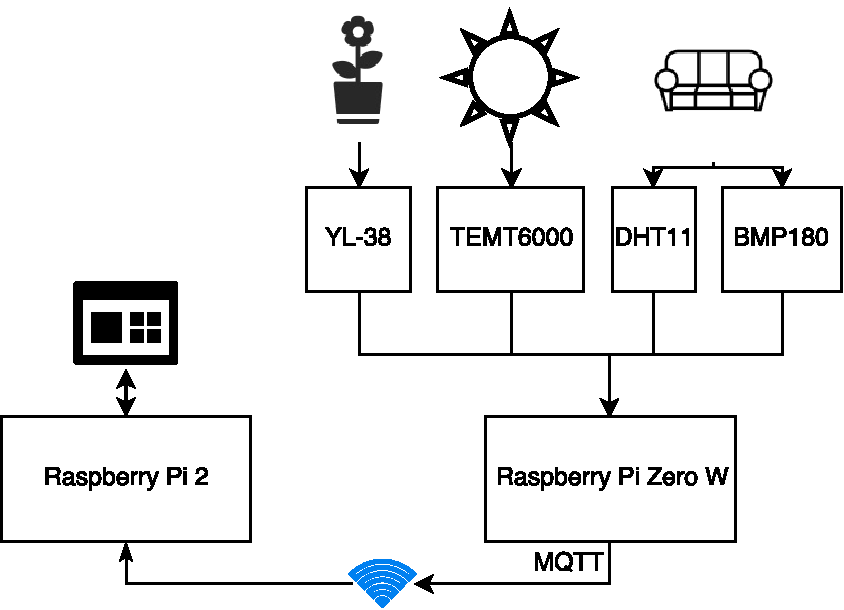
\includegraphics[width=0.5\linewidth]{weather-station-scheme}
    \caption{Schéma zapojení hardware.}
\end{figure}

\subsection{Software}\label{subsec:sw}
Na obrázku~\ref{fig:sw-scheme} je znázorněné propojení jednotlivých modulů a způsob jejich komunikace.

\begin{figure}[htb]
    \centering
    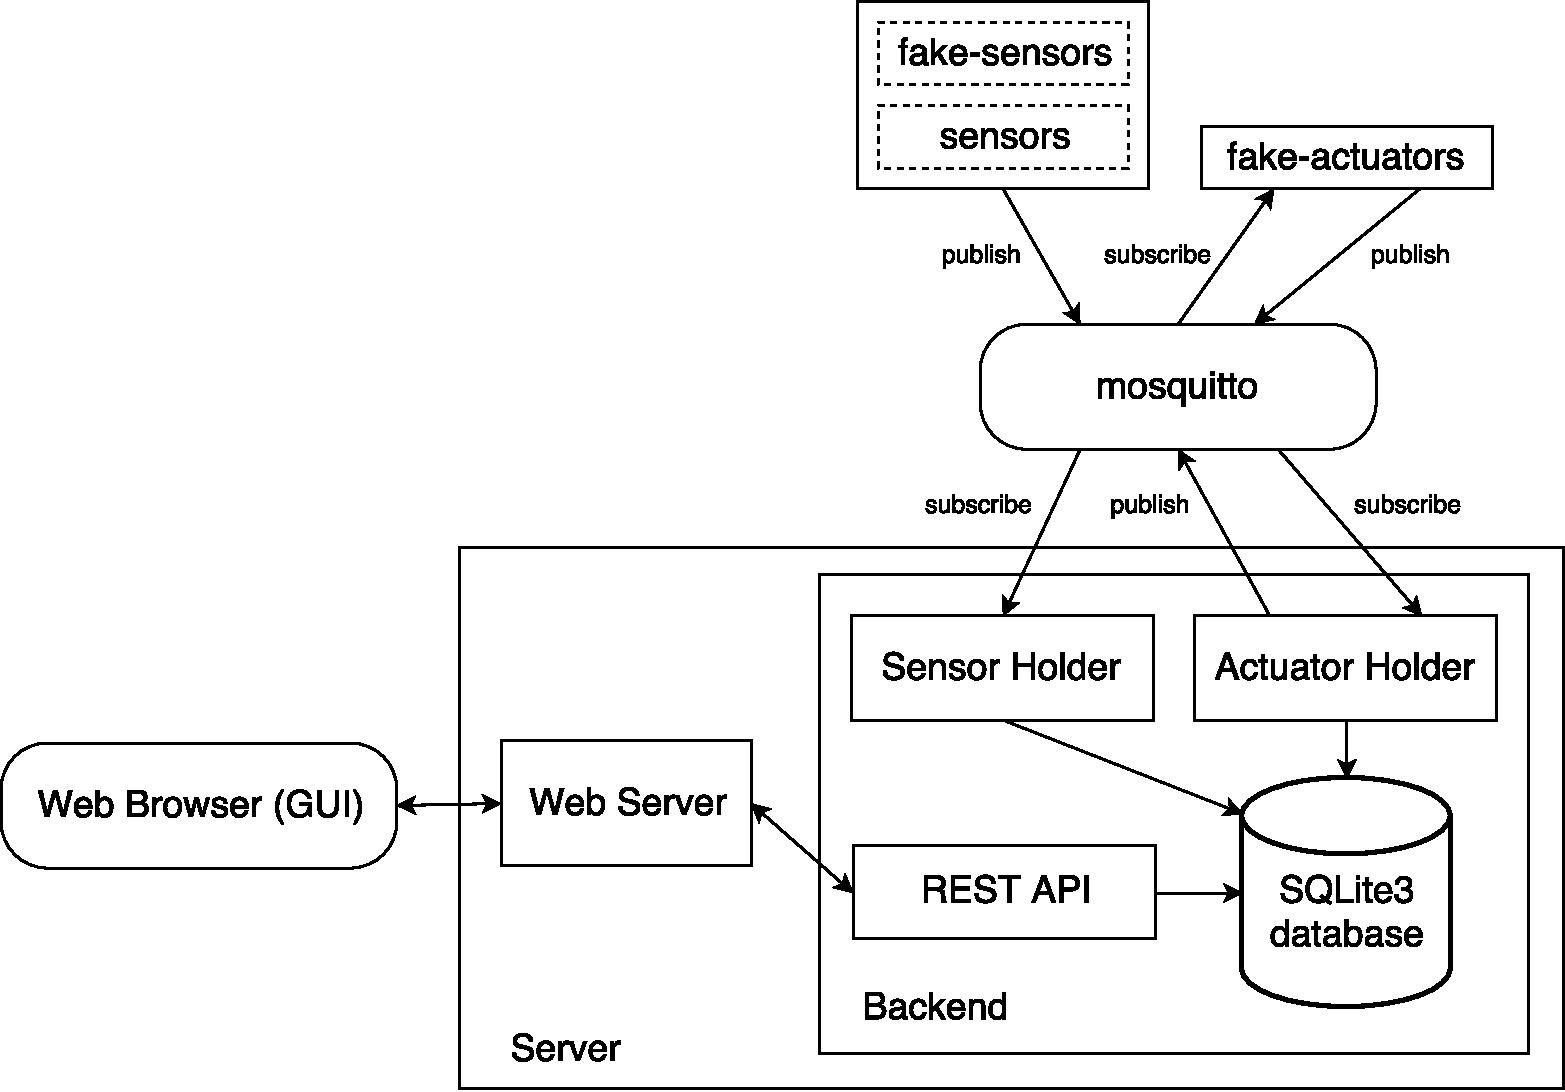
\includegraphics[width=0.75\linewidth]{sw-scheme}
    \caption{Schéma propojení software modulů.}
    \label{fig:sw-scheme}
\end{figure}

Interakci s uživatelem zprostředkovává webová aplikace, která se skládá z grafického uživatelského rozhraní zobrazovaného ve webovém prohlížeči a serverové části.

Webové grafické uživatelské rozhraní je naimplementované ve frameworku Angular. Webová aplikace dále využívá knihovnu Dygraphs pro zobrazování čárových grafů pro jednotlivé naměřené metriky. GUI získává data pomocí REST API ze serverové části aplikace. Při prvním načtení se získají historická data za posledních 24 hodin a dále si GUI získává nová data každých 5 sekund.

K implementaci REST API je použit framework Flask.
Serverová část webové aplikace (backend) přijímá data ze senzorů a ukládá je do databáze.
Na základě dat ze senzorů a nastavených pravidel určuje činnost a řídí aktuátorů.

REST API umožňuje:
\begin{itemize}
    \item získat poslední vzorek dat ze senzorů včetně časové známky spolu s trendem vypočítaným pro každou měřenou metriku
    \item získat informace o aktuálním stavu aktuátorů a pravidlech, kterými jsou řízeny
    \item nastavit nové prahové hodnoty jednotlivým aktuátorům
\end{itemize}

Výpočet trendů probíhá na základě lineární aproximace z určitého počtu posledních vzorků dané veličiny.
Pro každou veličinu je tak určena funkce ve tvaru:
\[
    y = a x + b
\]
Koeficient $a$ udává jako prudce funkce klesá nebo stoupá.
Koeficient $b$ udává posunutí funkce po ose $x$.
Toto posunutí nemá na změnu veličiny vliv a proto může být z dalších výpočtů vypuštěno.
Do vztahu:
\[
    y = a x
\]
je potom za $x$ dosazený počet vzorků, z kterých sa počítá trend.
Hodnota $y$ udáva o kolik sa daná veličina za posledních $x$ vzorků změnila.

Pro každou veličinu byly empirickým pozorováním určené hodnoty prahů.
Pokud je absolutní hodnota změny veličiny větší než práh, tak podle znaménka změny veličiny je určen stoupající nebo klesající trend, jinak je určen trend rovnoměrného průběhu.

V databázi SQLite3 sa nachází 3 tabulky:
\begin{itemize}
    \item \texttt{weather\_data} - data získaná ze senzorů
    \item \texttt{actuators} - informace o stavu aktuátorů
    \item \texttt{thresholds} - informace o pravidlech řídících činnost aktuátorů
\end{itemize}

Data ze senzorů získává, agreguje a následně odesílá backendu modul \texttt{sensors}.
Pro testovací účely byl připraven i modul \texttt{fake-sensors}, který simuluje
činnost modulu \texttt{sensors} a odesílá umělá data ve stejném formátu.

Modul \texttt{fake-actuators} simuluje činnost aktuátorů.
Z backendu přijímá příkazy na změnu stavu aktuátorů, které simuluje.
Po provedení činnosti aktuátorů je odeslána informace o stavu, ve kterém
se aktuátor nachází backendu.

Následuje seznam simulovaných aktuátorů:
\begin{itemize}
    \item klimatizace - řízená na základě údajů o teplotě
    \item topení - řízené na základě údajů o teplotě
    \item žaluzie - řízené na základě údajů o intenzitě světla
    \item zavlažování rostlin - řízené na základě údajů o vlhkosti půdy
\end{itemize}

Komunikace mezi backendem, senzory a aktuátory probíhá skrz protokol MQTT. Jako broker byl zvolen nástroj Mosquitto.

MQTT topic pro zprávy zasílané senzory má tvar \texttt{home/ws/sensor/<jméno senzoru>} a obsah dané zprávy ve formátu \texttt{<unix časové razítko>;<hodnota>}.

MQTT topic pro zprávy zasílané aktuátory má tvar \texttt{home/ws/actuator/<jméno senzoru>} a obsah dané zprávy ve stejném formátu jako u senzorů.

Aktuátory přijímají MQTT zprávy od backendu pro nastavení stavu s MQTT topic ve tvaru: \texttt{home/ws/actuator/<jméno senzoru>/state} a obsahem zprávy je pouze nově nastavovaná hodnota v podobě hodnoty 0 nebo 1.

\section{Demonstrace systému}\label{sec:res}
Celý systém lze spustit v demonstračním režimu, v kterém je simulována činnost aktuátorů i senzorů. Prerekvizity pro spuštení demostrace systémů pomocí skriptu \texttt{run.sh} jsou:
\begin{itemize}
    \item Python 2.7
    \item moduly pip a virtualenv
    \item NodeJS 8.7 a npm 5.4
    \item Angular CLI 1.4.1\footnote{Balik Angular CLI vyžaduje globalní instalaci příkazem npm i \texttt{@angular/cli@1.4.1 -g}}
    \item spuštěný Mosquitto broker na výchozím portu 1883
    \item dostupné a volné porty 4200 a 8080
\end{itemize}
Postup pro demonstraci systému je následující:
\begin{enumerate}
    \item spustit bash skript \texttt{run.sh}
    \item otevřít webový prohlížeč na adrese \url{http://localhost:4200}
\end{enumerate}

\section{Závěr}\label{sec:sum}
Webová aplikace pro vytvořený systém, která obsahuje data naměřená z reálných aktivních senzorů a simulovaných aktuátorů, je dostupná z adresy \url{https://ws.petrstehlik.cz}. Pro demonstrační účely byl vytvořen skript, který nainstaluje potřebné nástroje pro backend i frontend a spustí frontend, backend a moduly pro simulaci činnosti aktuátorů a senzorů.

\end{document}
